\documentclass[10pt,aspectratio=169]{beamer}

% Cấu hình theme
\usetheme{Madrid}
\usecolortheme{default}
\usefonttheme{professionalfonts} % Sử dụng font chuyên nghiệp hơn
\setbeamerfont{caption}{size=\scriptsize}

% Gói hỗ trợ tiếng Việt và các gói khác
\usepackage[utf8]{vietnam}
\usepackage[utf8]{inputenc}
\usepackage[T5]{fontenc}
\usepackage{lmodern} % Font Latin Modern sắc nét hơn
\usepackage[scaled]{helvet} % Dùng font Helvetica (giống Arial) làm font chính
\renewcommand{\familydefault}{\sfdefault} % Chắc chắn dùng sans-serif

\usepackage{bookmark}
\usepackage{graphicx}
\usepackage{booktabs}
\usepackage{algorithm}
\usepackage{algpseudocode}
\usepackage{listings}
\usepackage{xcolor}
\usepackage{tikz}
\usepackage{multirow}
\usepackage{array}
\usetikzlibrary{shapes,arrows,positioning,fit,calc}

% Cấu hình code block đẹp hơn

\lstset{
    language=Python,
    basicstyle=\ttfamily\scriptsize, % Tăng size lên xíu cho dễ nhìn
    keywordstyle=\color{blue}\bfseries,
    commentstyle=\color{green!50!black}\itshape, % Comment in nghiêng, màu dịu hơn
    stringstyle=\color{orange!80!black},
    identifierstyle=\color{black},
    breaklines=true,
    frame=shadowbox, % Khung bóng đổ đẹp hơn
    rulesepcolor=\color{gray},
    showstringspaces=false,
    numbers=left,
    numberstyle=\tiny\color{gray},
    numbersep=5pt,
    tabsize=4,
    backgroundcolor=\color{yellow!5}, % Nền code màu nhạt dễ đọc
    escapeinside={(*@}{@*)}
}

% Định nghĩa lại tên thuật toán
\floatname{algorithm}{Thuật toán}
\renewcommand{\algorithmicrequire}{\textbf{Input:}}
\renewcommand{\algorithmicensure}{\textbf{Output:}}

% --- ĐỊNH NGHĨA TRANG BÌA CUSTOM (MINIMALIST WHITE) ---
\setbeamertemplate{title page}{
    \begin{tikzpicture}[remember picture,overlay]
        % Thanh màu xanh mỏng ở trên cùng
        \fill[structure.fg] (current page.north west) rectangle ([yshift=-0.2cm]current page.north east);
    \end{tikzpicture}
    
    \vspace{1.5cm}
    
    % Dòng tên trường
    {\tiny\bfseries\color{structure.fg!80} TRƯỜNG ĐẠI HỌC XÂY DỰNG HÀ NỘI \\ KHOA CÔNG NGHỆ THÔNG TIN \par}
    
    \vspace{0.5cm}
    
    % Tiêu đề chính (Font Serif to, đậm - Đã giảm size theo yêu cầu)
    {\usefont{T5}{put}{b}{n}\fontsize{16}{22}\selectfont\textcolor{black}{Ứng dụng thuật toán Eclat trong phân tích hành vi người dùng qua dữ liệu clickstream để gợi ý nội dung}\par}
    
    \vspace{0.3cm}
    
    % Subtitle
    {\color{gray} Báo cáo Bài tập lớn môn Khai phá dữ liệu \par}
    
    \vspace{1.5cm} 
    
    % Cột thông tin (Giảng viên & Sinh viên)
    \begin{columns}[t]
        \column{0.45\textwidth}
            {\scriptsize\bfseries\color{structure.fg} GIẢNG VIÊN HƯỚNG DẪN}\\[0.1cm]
            {\large\bfseries TS. Phạm Hồng Phong}
            
        \column{0.55\textwidth}
            {\scriptsize\bfseries\color{structure.fg} NHÓM THỰC HIỆN}\\[0.1cm]
            {\small
            1. Nguyễn Việt Anh (0203968)\\
            2. Nguyễn Việt Hùng (0208768)\\
            3. Đỗ Quang Hợp (0208568)
            }
    \end{columns}
    
    \vfill
}

% Thông tin Metadata
\title[Thuật toán Eclat]{Ứng dụng thuật toán Eclat trong phân tích hành vi\\người dùng qua dữ liệu clickstream để gợi ý nội dung}

\author[Việt Anh - Việt Hùng - Quang Hợp]{
    Nguyễn Việt Anh \and Nguyễn Việt Hùng \and Đỗ Quang Hợp
}
\institute[ĐH Xây Dựng HN]{
    Khoa Công nghệ Thông tin \\
    Trường Đại học Xây Dựng Hà Nội
}
\date{Tháng 2 năm 2026}

\begin{document}

% Slide 1: Trang bìa
\begin{frame}
    \titlepage
\end{frame}

% Slide 2: Mục lục
\begin{frame}{Nội dung trình bày}
    \tableofcontents
\end{frame}

% ============================================================
% CHƯƠNG 1: TỔNG QUAN
% ============================================================
\section{Tổng quan đề tài}

\begin{frame}{Đặt vấn đề}
    \textbf{Bối cảnh thực tế:}
    \begin{itemize}
        \item Sự bùng nổ dữ liệu hành vi người dùng (clickstream data) trên các website/ứng dụng.
        \item Phân tích dữ liệu này giúp: Hiểu hành vi người dùng, tối ưu UX, tăng doanh thu.
    \end{itemize}

    \vspace{0.5cm}
    \textbf{Giải pháp - Khai phá luật kết hợp:}
    \begin{itemize}
        \item Tìm kiếm các mối quan hệ tiềm ẩn giữa các mục trong tập dữ liệu lớn.
        \item Ví dụ kinh điển: "Bia và Tã lót".
    \end{itemize}
\end{frame}

\begin{frame}{Mục tiêu đề tài}
    \begin{enumerate}
        \item \textbf{Nghiên cứu \& Triển khai}: Thuật toán \textbf{Eclat} từ đầu (from scratch), không dùng thư viện có sẵn.
        \item \textbf{Ứng dụng thực tế}: Phân tích dữ liệu clickstream từ \textbf{MSNBC.com} (gần 1 triệu giao dịch).
        \item \textbf{Sinh luật gợi ý}: Dạng \textit{"Nếu xem A $\rightarrow$ Gợi ý B"}.
        \item \textbf{Đánh giá}: Sử dụng các chỉ số Support, Confidence, Lift.
    \end{enumerate}
\end{frame}

\begin{frame}{Phạm vi nghiên cứu}
    \begin{itemize}
        \item \textbf{Dữ liệu}: MSNBC.com Anonymous Web Data (UCI Machine Learning Repository).
        \item \textbf{Thuật toán}: Eclat (Equivalence Class Transformation) [Zaki, 2000].
        \item \textbf{Công nghệ}: Python 3.x.
        \item \textbf{Phương pháp}: Cài đặt thủ công cấu trúc dữ liệu và giải thuật.
    \end{itemize}
\end{frame}

% ============================================================
% CHƯƠNG 2: CƠ SỞ LÝ THUYẾT
% ============================================================
\section{Cơ sở lý thuyết}

\begin{frame}{Khai phá luật kết hợp}
    \begin{block}{Các khái niệm cơ bản}
        \begin{itemize}
            \item \textbf{Itemset (Tập mục)}: Tập hợp các mục, ví dụ $X = \{A, B\}$.
            \item \textbf{Support (Độ hỗ trợ)}: Tỷ lệ xuất hiện của itemset trong CSDL.
            \[ Support(X) = \frac{|\{T \in D : X \subseteq T\}|}{|D|} \]
            \item \textbf{Frequent Itemset}: Itemset có $Support \geq min\_support$.
            \item \textbf{Luật kết hợp}: $X \Rightarrow Y$ ("Nếu $X$ thì $Y$").
        \end{itemize}
    \end{block}
\end{frame}

\begin{frame}{Các chỉ số đánh giá luật}
    \begin{columns}[t]
        \column{0.5\textwidth}
            \textbf{1. Confidence (Độ tin cậy)}
            \[ Conf(X \Rightarrow Y) = \frac{Sup(X \cup Y)}{Sup(X)} \]
            \begin{itemize}
                \item Xác suất có điều kiện $P(Y|X)$.
                \item Đo lường độ "chắc chắn" của luật.
            \end{itemize}
        
        \column{0.5\textwidth}
            \textbf{2. Lift (Độ tương quan)}
            \[ Lift = \frac{Sup(X \cup Y)}{Sup(X) \times Sup(Y)} \]
            \begin{itemize}
                \item $>1$: Tương quan dương (Tốt).
                \item $=1$: Độc lập.
                \item $<1$: Tương quan âm.
            \end{itemize}
    \end{columns}
\end{frame}

% --- VÍ DỤ MINH HỌA THEO BÁO CÁO ---


\begin{frame}{Thuật toán Eclat: Tổng quan}
    \textbf{Eclat} (Equivalence Class Transformation)
    \begin{itemize}
        \item Đề xuất: \textbf{Mohammed J. Zaki} (2000).
        \item Là thuật toán khai phá tập phổ biến (Frequent Itemset Mining) hiệu quả cao.
        \item \textbf{Tư tưởng chính:} Thay vì đếm số lần xuất hiện (như Apriori), Eclat sử dụng \textbf{giao của các tập định danh giao dịch (Intersection of TID-Sets)}.
    \end{itemize}
    
    \vspace{0.5cm}
    \textbf{Chiến lược tìm kiếm:}
    \begin{enumerate}
        \item \textbf{Vertical Data Format}: Chuyển đổi dữ liệu sang dạng dọc.
        \item \textbf{DFS (Depth-First Search)}: Duyệt theo chiều sâu để tìm tập phổ biến.
    \end{enumerate}
\end{frame}

\begin{frame}{1. Định dạng dữ liệu (Data Format)}
    \begin{columns}[t]
        \column{0.48\textwidth}
            \textbf{A. Horizontal Format (Truyền thống)}
            \begin{table}\centering\scriptsize
            \begin{tabular}{|c|l|}
            \hline \textbf{TID} & \textbf{Items} \\ \hline
            1 & A, B, C \\
            2 & A, B \\
            3 & A, C \\
            \hline \end{tabular}
            \end{table}
            
            \begin{alertblock}{Vấn đề}
                Để biết \textbf{\{A, B\}} xuất hiện bao nhiêu lần:
                \begin{itemize}
                    \item Phải quét từng dòng (Scan DB).
                    \item Kiểm tra: Dòng 1 có A, B? (Có) $\rightarrow$ +1.
                    \item Dòng 2 có A, B? (Có) $\rightarrow$ +1.
                \end{itemize}
                $\Rightarrow$ \textbf{Rất tốn kém (Expensive Scans)}.
            \end{alertblock}
        
        \column{0.48\textwidth}
            \textbf{B. Vertical Format (Eclat)}
            \begin{table}\centering\scriptsize
            \begin{tabular}{|c|l|}
            \hline \textbf{Item} & \textbf{TID-Set (Ai mua?)} \\ \hline
            A & \{1, 2, 3\} \\
            B & \{1, 2\} \\
            C & \{1, 3\} \\
            \hline \end{tabular}
            \end{table}
            
            \begin{exampleblock}{Giải pháp của Eclat}
                Để biết \textbf{\{A, B\}} xuất hiện bao nhiêu lần:
                \begin{itemize}
                    \item Lấy TID(A) giao TID(B).
                    \item $\{1,2,3\} \cap \{1,2\} = \{1,2\}$.
                    \item Đếm kích thước = 2.
                \end{itemize}
                $\Rightarrow$ \textbf{Tính toán tức thì (Instant Calculation)}.
            \end{exampleblock}
    \end{columns}
\end{frame}

\begin{frame}{2. Nguyên lý hoạt động cốt lõi}
    \begin{columns}
        \column{0.5\textwidth}
        \textbf{Cơ sở toán học:}
        \begin{itemize}
            \item Eclat dựa trên lý thuyết tập hợp (Set Theory).
            \item Thay vì \textit{kiểm tra} từng giao dịch xem có chứa A và B không (Scan), ta \textit{xác định} giao dịch đó bằng cách lấy phần chung của tập TID.
            \item \textbf{Định lý}: Tập hợp các giao dịch chứa itemset $X \cup Y$ chính là giao của tập TID chứa $X$ và tập TID chứa $Y$.
            \[ TID(XY) = TID(X) \cap TID(Y) \]
        \end{itemize}

        \column{0.5\textwidth}
        \centering
        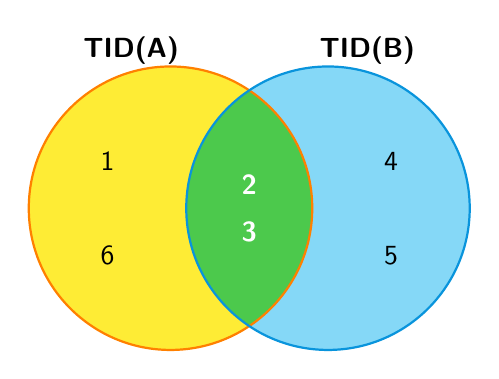
\begin{tikzpicture}[thick]
            % Tô màu Vòng tròn A (Vàng) - Nguyên khối
            \fill[yellow!90!orange, opacity=0.8] (-1,0) circle (1.8cm);
            
            % Tô màu Vòng tròn B (Xanh Cyan) - Nguyên khối
            \fill[cyan!60, opacity=0.8] (1,0) circle (1.8cm);

            % Tô lại màu phần giao (Xanh lá) 
            % Dùng clip để chỉ tô phần giao nhau
            \begin{scope}
                \clip (-1,0) circle (1.8cm);
                \fill[green!70!black!70] (1,0) circle (1.8cm);
            \end{scope}

            % Vẽ viền 2 vòng tròn (Vẽ sau cùng để đè lên màu tô)
            \draw[orange, thick] (-1,0) circle (1.8cm);
            \draw[cyan!80!blue, thick] (1,0) circle (1.8cm);

            % Label
            \node at (-1.5, 2) {\textbf{TID(A)}};
            \node at (1.5, 2) {\textbf{TID(B)}};

            % Nội dung bên trong (Số) - Căn chỉnh vị trí để không bị lẹm vào phần giao
            \node at (-1.8, 0.6) {1};
            \node at (-1.8, -0.6) {6};
            
            \node at (1.8, 0.6) {4};
            \node at (1.8, -0.6) {5};

            % Phần giao (Màu chữ trắng)
            \node at (0, 0.3) {\textbf{\textcolor{white}{2}}};
            \node at (0, -0.3) {\textbf{\textcolor{white}{3}}};
        \end{tikzpicture}
        \\
        \footnotesize \textit{Màu xanh lá thể hiện tập giao nhau (Intersection)}
    \end{columns}
    
    \vspace{0.2cm}
    \textbf{Kết luận từ hình:}
    \begin{itemize}
        \item $TID(A) = \{1, 2, 3, 6\}$ (Có 4 phần tử $\rightarrow$ \textbf{Sup=4})
        \item $TID(B) = \{2, 3, 4, 5\}$ (Có 4 phần tử $\rightarrow$ \textbf{Sup=4})
        \item $\rightarrow TID(A \cap B) = \{\textbf{2, 3}\}$ (Còn 2 phần tử $\rightarrow$ \textbf{Sup=2})
    \end{itemize}
    \textit{*Sup (Support Count): Số lượng giao dịch chứa item.}
\end{frame}

\begin{frame}{3. Quy trình thực hiện (Workflow)}
    \begin{enumerate}
        \item \textbf{Bước 1: Khởi tạo (Initialization)}
        \begin{itemize}
            \item Quét CSDL \textbf{1 lần duy nhất} để chuyển đổi sang định dạng dọc (Vertical Format).
            \item Lọc bỏ các item không phổ biến (có độ hỗ trợ $< min\_support$) ngay từ đầu để giảm không gian tìm kiếm.
        \end{itemize}
        \vspace{0.3cm}
        
        \item \textbf{Bước 2: Tìm kiếm đệ quy (Recursive Search - DFS)}
        \begin{itemize}
            \item Với mỗi itemset $P$ (prefix), kết hợp với các itemset item $Q_i$ khác.
            \item Tính tập TID mới bằng phép giao: $TID(P \cup Q_i) = TID(P) \cap TID(Q_i)$.
            \item Nếu kích thước tập TID mới $\ge min\_support$: 
            \begin{itemize}
                \item Lưu itemset $\{P, Q_i\}$ là tập phổ biến.
                \item Tiếp tục gọi đệ quy với prefix mới là $\{P, Q_i\}$.
            \end{itemize}
        \end{itemize}
        \vspace{0.3cm}
        
        \item \textbf{Bước 3: Kết thúc (Termination)}
        \begin{itemize}
            \item Quá trình dừng lại khi không còn cặp item nào để kết hợp hoặc tập giao kết quả rỗng.
            \item Thuật toán quay lui (backtrack) để xét các nhánh khác.
        \end{itemize}
    \end{enumerate}
\end{frame}



% --- Slide Ví dụ 1: Input & Bước 1 ---
\begin{frame}{Ví dụ minh họa thuật toán Eclat}
    \textbf{Giả thiết:} 4 giao dịch, $min\_support = 50\%$ (xuất hiện $\ge 2$ lần).
    
    \textbf{Dữ liệu đầu vào:}
    \begin{table}\centering\small
    \begin{tabular}{|c|l|}
    \hline \textbf{TID} & \textbf{Items} \\ \hline
    1 & A, B, C \\
    2 & B, C, D \\
    3 & A, C, D \\
    4 & A, B, D \\
    \hline \end{tabular}
    \end{table}

    \textbf{Bước 1: Chuyển sang Vertical Format (TID-Sets của 1-itemset)}
    \begin{table}\centering\small
    \begin{tabular}{|c|l|c|c|}
    \hline \textbf{Item} & \textbf{TID-Set} & \textbf{Count} & \textbf{Support} \\ \hline
    A & \{1, 3, 4\} & 3 & 75\% \\
    B & \{1, 2, 4\} & 3 & 75\% \\
    C & \{1, 2, 3\} & 3 & 75\% \\
    D & \{2, 3, 4\} & 3 & 75\% \\
    \hline \end{tabular}
    \end{table}
    $\Rightarrow$ Tất cả đều thỏa mãn $\ge 50\%$.
\end{frame}

% --- Slide Ví dụ 2: Bước 2 & Bước 3 ---
\begin{frame}{Ví dụ minh họa: Tính toán các Itemsets lớn hơn}
    \textbf{Bước 2: Tính TID-Sets cho 2-itemsets (bằng phép giao)}
    \begin{table}\centering\scriptsize
    \begin{tabular}{|c|c|c|c|l|}
    \hline \textbf{Itemset} & \textbf{Phép giao} & \textbf{TID-Set} & \textbf{Count} & \textbf{Kết luận} \\ \hline
    \{A, B\} & \{1,3,4\} $\cap$ \{1,2,4\} & \{1, 4\} & 2 & Có (50\%) \\
    \{A, C\} & \{1,3,4\} $\cap$ \{1,2,3\} & \{1, 3\} & 2 & Có (50\%) \\
    \{A, D\} & \{1,3,4\} $\cap$ \{2,3,4\} & \{3, 4\} & 2 & Có (50\%) \\
    \{B, C\} & \{1,2,4\} $\cap$ \{1,2,3\} & \{1, 2\} & 2 & Có (50\%) \\
    \{B, D\} & \{1,2,4\} $\cap$ \{2,3,4\} & \{2, 4\} & 2 & Có (50\%) \\
    \{C, D\} & \{1,2,3\} $\cap$ \{2,3,4\} & \{2, 3\} & 2 & Có (50\%) \\
    \hline \end{tabular}
    \end{table}

    \textbf{Bước 3: Tính TID-Sets cho 3-itemsets}
    \begin{table}\centering\scriptsize
    \begin{tabular}{|c|c|c|c|l|}
    \hline \textbf{Itemset} & \textbf{Phép giao} & \textbf{TID-Set} & \textbf{Count} & \textbf{Kết luận} \\ \hline
    \{A, B, C\} & \{1,4\} $\cap$ \{1,2,3\} & \{1\} & 1 & Không (25\%) \\
    \{A, B, D\} & \{1,4\} $\cap$ \{2,3,4\} & \{4\} & 1 & Không (25\%) \\
    \{A, C, D\} & \{1,3\} $\cap$ \{2,3,4\} & \{3\} & 1 & Không (25\%) \\
    \{B, C, D\} & \{1,2\} $\cap$ \{2,3,4\} & \{2\} & 1 & Không (25\%) \\
    \hline \end{tabular}
    \end{table}
    $\Rightarrow$ Không có 3-itemset nào đạt ngưỡng, thuật toán dừng.
\end{frame}

% --- Slide Ví dụ 3: Tổng kết ---
\begin{frame}{Ví dụ minh họa: Bước 4 - Tổng kết kết quả}
    \textbf{Bảng tổng hợp tất cả Frequent Itemsets ($min\_support = 50\%$)}
    
    \vspace{0.5cm}
    \begin{table}\centering
    \begin{tabular}{|c|l|c|}
    \hline \textbf{Kích thước} & \textbf{Frequent Itemsets} & \textbf{Số lượng} \\ \hline
    1-itemset & \{A\}, \{B\}, \{C\}, \{D\} & 4 \\ \hline
    2-itemset & \{A,B\}, \{A,C\}, \{A,D\}, \{B,C\}, \{B,D\}, \{C,D\} & 6 \\ \hline
    \textbf{Tổng} & \textbf{Tổng cộng} & \textbf{10} \\ \hline
    \end{tabular}
    \end{table}
\end{frame}

\begin{frame}[fragile]{Mã giả thuật toán Eclat}
    \scriptsize
    \begin{algorithmic}[1]
        \State \textbf{Đầu vào:} Cơ sở dữ liệu $D$, ngưỡng $min\_support$
        \State \textbf{Đầu ra:} Tập hợp tất cả các Frequent Itemsets $F$
        \State $F \gets \emptyset$
        \State $min\_support\_count \gets |D| \times min\_support$
        \State Chuyển đổi $D$ sang định dạng dọc: $TID\_Dict$
        \State Lọc các 1-itemsets có $|TID| < min\_support\_count$
        \State Sắp xếp $TID\_Dict$ theo $|TID|$ giảm dần
        
        \Procedure{ECLAT\_RECURSIVE}{$Prefix, TID\_Subset, min\_support\_count$}
            \While{$TID\_Subset \neq \emptyset$}
                \State $(item, tids) \gets TID\_Subset.pop(0)$ \Comment{Lấy phần tử đầu}
                \State $NewItemset \gets Prefix \cup \{item\}$
                \State $F \gets F \cup \{(NewItemset, |tids|)\}$ \Comment{Lưu kết quả}
                
                \State $NewSubset \gets \emptyset$
                \ForAll{$(other\_item, other\_tids) \in TID\_Subset$}
                    \State $IntersectTids \gets tids \cap other\_tids$ \Comment{Phép giao}
                    \If{$|IntersectTids| \ge min\_support\_count$}
                        \State $NewSubset \gets NewSubset \cup \{(other\_item, IntersectTids)\}$
                    \EndIf
                \EndFor
                
                \If{$NewSubset \neq \emptyset$}
                    \State \Call{ECLAT\_RECURSIVE}{$NewItemset, NewSubset, min\_support\_count$}
                \EndIf
            \EndWhile
        \EndProcedure
        
        \State \Call{ECLAT\_RECURSIVE}{$\emptyset, TID\_Dict, min\_support\_count$}
        \State \Return $F$
    \end{algorithmic}
\end{frame}



% ============================================================
% CHƯƠNG 3: DỮ LIỆU VÀ TIỀN XỬ LÝ
% ============================================================
\section{Dữ liệu và Tiền xử lý}

\begin{frame}{Giới thiệu bộ dữ liệu MSNBC}
    \begin{itemize}
        \item \textbf{Nguồn}: UCI Machine Learning Repository.
        \item \textbf{Thời gian}: 28/09/1999 từ MSNBC.com.
        \item \textbf{Thống kê}:
        \begin{itemize}
            \item Tổng số phiên: \textbf{989,818}.
            \item Số chuyên mục: \textbf{17}.
            \item Trung bình click/phiên: 5.7.
        \end{itemize}
        \item \textbf{Cấu trúc}: File .seq, mỗi dòng là một phiên truy cập chứa các ID chuyên mục.
    \end{itemize}
\end{frame}

\begin{frame}{Ánh xạ dữ liệu (Mapping)}
    \begin{table}
    \centering\small
    \renewcommand{\arraystretch}{1.2}
    \begin{tabular}{|c|l|c|l|}
    \hline \textbf{ID} & \textbf{Tên chuyên mục} & \textbf{ID} & \textbf{Tên chuyên mục} \\ \hline
    1 & Trang chủ (Frontpage) & 10 & Đời sống (Living) \\
    2 & Tin tức (News) & 11 & Kinh doanh (Business) \\
    3 & Công nghệ (Tech) & 12 & Thể thao (Sports) \\
    4 & Địa phương (Local) & 13 & Tóm tắt (Summary) \\
    5 & Ý kiến (Opinion) & 14 & Diễn đàn (BBS) \\
    6 & Phát sóng (On-air) & 15 & Du lịch (Travel) \\
    7 & Tổng hợp (Misc) & 16 & Tin MSN (MSN-News) \\
    8 & Thời tiết (Weather) & 17 & Thể thao MSN (MSN-Sports) \\
    9 & Sức khỏe (Health) & & \\
    \hline
    \end{tabular}
    \end{table}
\end{frame}

\begin{frame}{Quy trình tiền xử lý}
    \begin{enumerate}
        \item \textbf{Đọc file}: Bỏ qua metadata (\%).
        \item \textbf{Parse}: Tách ID số.
        \item \textbf{Mapping}: Chuyển ID $\rightarrow$ Tên chuyên mục.
        \item \textbf{Loại trùng lặp}: Sử dụng \texttt{set()} để mỗi chuyên mục chỉ xuất hiện 1 lần/phiên (vì Eclat chỉ quan tâm có/không).
        \item \textbf{Lọc rỗng}: Bỏ các phiên không hợp lệ.
    \end{enumerate}

    \vspace{0.3cm}
     \textbf{Lưu ý:} Việc dùng \texttt{set()} giúp giảm kích thước dữ liệu và tăng tốc độ xử lý.
\end{frame}

% ============================================================
% CHƯƠNG 4: TRIỂN KHAI THUẬT TOÁN
% ============================================================
\section{Triển khai thuật toán}

\begin{frame}{Kiến trúc hệ thống}
    \centering
    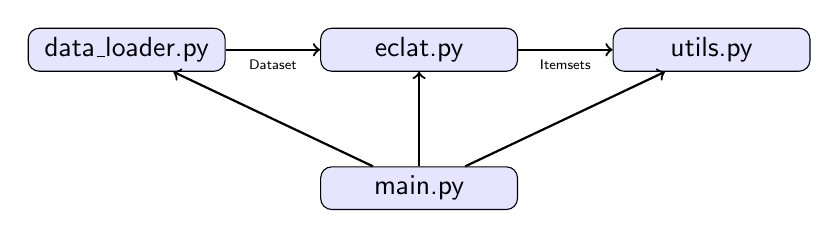
\begin{tikzpicture}[node distance=1.2cm, box/.style={rectangle, draw, rounded corners, fill=blue!10, text centered, minimum width=2.5cm}]
        \node[box] (data) {data\_loader.py};
        \node[box, right=of data] (algo) {eclat.py};
        \node[box, right=of algo] (utils) {utils.py};
        \node[box, below=of algo] (main) {main.py};
        
        \draw[->, thick] (main) -- (data);
        \draw[->, thick] (main) -- (algo);
        \draw[->, thick] (main) -- (utils);
        \draw[->, thick] (data) -- (algo) node[midway, below]{\tiny Dataset};
        \draw[->, thick] (algo) -- (utils) node[midway, below]{\tiny Itemsets};
    \end{tikzpicture}
    
    \vspace{0.5cm}
    \begin{itemize}
        \item \textbf{data\_loader.py}: Đọc và tiền xử lý dữ liệu.
        \item \textbf{eclat.py}: Cài đặt class Eclat và thuật toán đệ quy.
        \item \textbf{utils.py}: Sinh luật từ tập phổ biến.
        \item \textbf{main.py}: File chạy chính.
    \end{itemize}
\end{frame}

\begin{frame}[fragile]{Cài đặt Eclat (Python)}
    \begin{lstlisting}
def _eclat_recursive(self, prefix, items, min_sup):
    while items:
        # Lay item dau tien (Pop)
        item, tids = items.pop(0)
        new_itemset = prefix + [item]
        
        # Luu ket qua
        if len(new_itemset) >= self.min_items:
            self.frequent_itemsets.append((new_itemset, len(tids)))
        
        # Tao danh sach ung vien tiep theo (Intersection)
        next_items = []
        for other_item, other_tids in items:
            new_tids = tids & other_tids  # Giao
            
            if len(new_tids) >= min_sup:  # Cat tia
                next_items.append((other_item, new_tids))
        
        # De quy DFS
        if next_items:
            self._eclat_recursive(new_itemset, next_items, min_sup)
    \end{lstlisting}
\end{frame}

% ============================================================
% CHƯƠNG 5: KẾT QUẢ VÀ ĐÁNH GIÁ
% ============================================================
\section{Kết quả và đánh giá}

\begin{frame}{Cấu hình và Kết quả tổng quan}
    \textbf{Cấu hình thực nghiệm:}
    \begin{itemize}
        \item Dữ liệu: Toàn bộ 989,818 phiên.
        \item Min Support: \textbf{0.02 (2\%)}.
        \item Min Confidence: \textbf{0.40 (40\%)}.
    \end{itemize}

    \vspace{0.3cm}
    \textbf{Kết quả:}
    \begin{itemize}
        \item 1-itemsets phổ biến: 15/17.
        \item 2-itemsets phổ biến: 17 cặp.
        \item \textbf{Tổng số tập phổ biến: 32}.
    \end{itemize}
    
    \textbf{Top chuyên mục:} Frontpage (95\%), News (45\%), Weather (44\%).
\end{frame}

\begin{frame}{Top 5 Luật gợi ý mạnh nhất}
    \begin{table}
    \centering\footnotesize
    \begin{tabular}{|c|l|l|c|c|c|}
    \hline
    \textbf{\#} & \textbf{Nếu xem} & \textbf{Gợi ý} & \textbf{Support} & \textbf{Conf.} & \textbf{Lift} \\
    \hline
    1 & Tổng hợp & Phát sóng & 3.36\% & 41.3\% & \textbf{1.88} \\
    2 & Kinh doanh & Trang chủ & 3.31\% & \textbf{56.8\%} & 1.80 \\
    3 & Đời sống & Trang chủ & 2.65\% & 51.9\% & 1.64 \\
    4 & Tổng hợp & Trang chủ & 3.68\% & 45.2\% & 1.43 \\
    5 & Tin tức & Trang chủ & 7.55\% & 42.6\% & 1.35 \\
    \hline
    \end{tabular}
    \end{table}
    
    \textit{(Đã lọc lift > 1 để đảm bảo tương quan dương)}
\end{frame}

\begin{frame}{Phân tích chi tiết}
    \textbf{1. Luật: Tổng hợp $\Rightarrow$ Phát sóng (Lift = 1.88)}
    \begin{itemize}
        \item \textbf{Insight}: Người xem tin tổng hợp rất thích xem video (Phát sóng). Xác suất xem video tăng gấp \textbf{1.88 lần} nếu họ đang ở mục Tổng hợp.
        \item \textbf{Gợi ý}: Nhúng widget Video vào trang Tổng hợp.
    \end{itemize}

    \vspace{0.3cm}
    \textbf{2. Luật: Kinh doanh $\Rightarrow$ Trang chủ (Conf = 56.8\%)}
    \begin{itemize}
        \item \textbf{Insight}: Hơn một nửa người đọc tin Kinh doanh sẽ quay lại Trang chủ.
        \item \textbf{Gợi ý}: Đặt nút "Về trang chủ" nổi bật hoặc banner tin nóng trên trang Kinh doanh.
    \end{itemize}
\end{frame}

% ============================================================
% CHƯƠNG 6: KẾT LUẬN
% ============================================================
\section{Kết luận}

\begin{frame}{Tổng kết}
    Đề tài đã đạt được các mục tiêu:
    \begin{itemize}
        \item[$\checkmark$] Hiểu và cài đặt thành công thuật toán \textbf{Eclat} (DFS, Vertical Format).
        \item[$\checkmark$] Xử lý hiệu quả tập dữ liệu lớn (~1 triệu dòng) từ MSNBC.
        \item[$\checkmark$] Tìm ra các luật có ý nghĩa (Lift > 1) để ứng dụng gợi ý nội dung.
    \end{itemize}
\end{frame}

\begin{frame}{Hạn chế và Hướng phát triển}
    \textbf{Hạn chế:}
    \begin{itemize}
        \item Dữ liệu cũ (1999).
        \item Mới chỉ xét cặp 2 chuyên mục (k=2).
    \end{itemize}

    \vspace{0.5cm}
    \textbf{Hướng phát triển:}
    \begin{itemize}
        \item \textbf{Sequential Mining}: Áp dụng GSP, PrefixSpan để xét đến \textit{thứ tự} click.
        \item \textbf{Real-time}: Tích hợp vào hệ thống gợi ý thời gian thực.
        \item \textbf{Demo}: Xây dựng giao diện Web App trực quan.
    \end{itemize}
\end{frame}

\begin{frame}
    \centering
    \Huge \textbf{CẢM ƠN THẦY VÀ CÁC BẠN\\ĐÃ LẮNG NGHE!}
    
    \vspace{1cm}
    \large \textbf{Q \& A}
\end{frame}

\end{document}
